\section{Electrical}
The electronics system is broken into the following two broad subsystems:
\begin{description}
 \item[Controller Circuitry] contains the radio link to the computers on the sidelines, and all motor control functionality.
 \item[Kicker Circuitry]  drives the kicker and chipper solenoids.
\end{description}
In comparison to the previous design revision, we added a chipper solenoid, but the charger and other switching mechanisms have remained largely the same. 

\begin{figure}
       \centering
       \vspace {0 cm}
       \includegraphics[height=0.3\textwidth]{images/elec}
       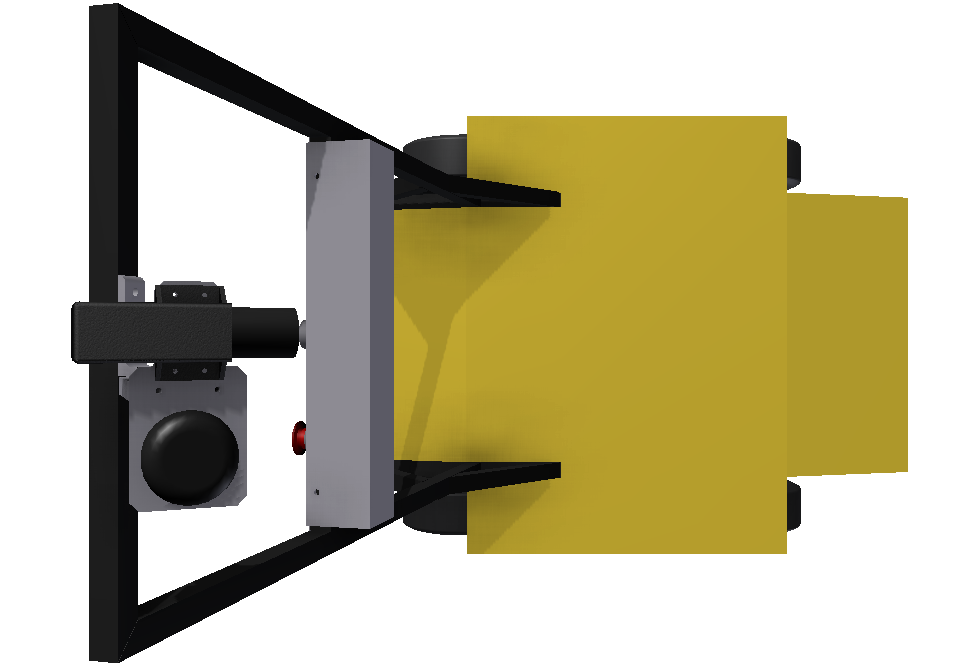
\includegraphics[height=0.3\textwidth]{images/top}
       \caption{Block diagram for the controller board (left), and a photograph of the actual board.}
\end{figure}

\subsection{Controller}
The primary functionality of the controller subsystem is to translate motor speeds sent by the computer on the sidelines to actual motor values. Though the controller is currently "dumb" we hope in the future to enable more intelligence on the robot.

The requirements of the electrical system derive from the requirements of the drive and dribbler motors. Each motor has three phases connected in a wye configuration and three hall effect sensors to establish rotor position. To drive a brushless motor the rotor position is used to determine which coils should be energized. A coil is energized with a half bridge. Each half bridge is composed of an N and P channel FET driven by a Microchip FET driver (TC4428). There are three half bridges per motor (one for each coil) for a total of 15 half bridges per robot. With miscellaneous passives, the motor driver circuitry composes about 150 components on each board. The half bridges are driven by a Xilinx 100K gate Spartan 3E (XC3S100E) FPGA. The FPGA is memory mapped to a NXP ARM7 (LPC2103) which handles local feedback control with information from US Digital encoders.

The robot communicates to the server via Texas Instruments CC1101 wireless ASSC. This ASSC allows tuning from 779MHz to 928MHz including the 868MHz ISM band. Packets from the radio modules are routed through the FPGA to the ARM to allow for future work in hardware accelerated wireless protocol research. Due to poor wireless performance in the previous year, and severe space constraints in the current design, standard monopole antennas were not used. Instead, a balanced dipole "halo" antenna will be utilized. The antenna is ideally suited for the challenge as it is very low profile and omnidirectional \cite{harrisonjr1961fda}.

In a typical design, power supplies and their distribution are normally considered a trivial implementation task. In contrast, this design has five power rails; 1V2, 1V8, 2V5, 3V3, and VBATT (12V). The many power rails present a considerable routing challenge. Despite this, the board is only two layers which affords much quicker and cheaper manufacturing then other processes. The 3V3 power supply is switching for high efficiency while the other lower voltages are produced with simple linear low dropout regulators.

\subsection{Kicker}
The kicker circuitry charges a bank of capacitors which are then discharged into the solenoids (both the kicker and the chipper) to kick the ball. The kicker uses a Linear Technologies LT3750 flyback controller to convert the battery voltage (12V) to approximately 250 volts which charges a 5400$\mu$F capacitor bank. The capacitors are discharged into the solenoids by means of an Insulated Gate Bipolar Transistor (IGBT). Ball speeds approaching legal limit have been achieved. In comparison to other designs, this design is quite compact, requiring only about three square inches of board area. This design also boasts efficiencies exceeding 80\%. 
